\documentclass[ucs]{beamer}
\usepackage{polski}
\usepackage[utf8]{inputenc}

%\usetheme{Ilmenau}
\usetheme{Marburg}

\title[Zależności czasowe w sieci EtherCAT]{Projekt i realizacja stanowiska laboratoryjnego do badania zależności czasowych w sieci EtherCAT}
\subtitle{The Desing and Application of a Laboratory Setup for Presentation of Temporal Parameters of EtherCAT Network}
\author{Damian Karbowiak}
\institute{Promotor: dr inż. Jacek Stój}
\date{\today}
\begin{document}

\begin{frame}
  \titlepage
\end{frame}

\section{Wstęp}
\begin{frame}
\frametitle{Opis}
Zakres pracy obejmuje projekt i realizację stanowiska laboratoryjnego złożonego z co najmniej dwóch sterowników produkcji Beckhoff do prezentacji zależności czasowych z sieci EtherCAT. Do tego celu oprócz sterowników należy użyć serwonapędów.
\end{frame}

\begin{frame}
\frametitle{Plan pracy}
\begin{enumerate}
    \item Zapoznanie się ze sterownikami Beckhoff oraz oprogramowaniem TwinCAT
    \item Zapoznanie się z dostępnymi serwonapędami Beckhoff
    \item Projekt i realizacja stanowiska
    \item Przygotowanie stanowiska do współpracy z systemem wizualizacji
    \item Testowanie i uruchamianie
\end{enumerate}
\end{frame}

\begin{frame}
\frametitle{Stanowisko typ 1}
\begin{figure}[!htb]	
\centering 	          
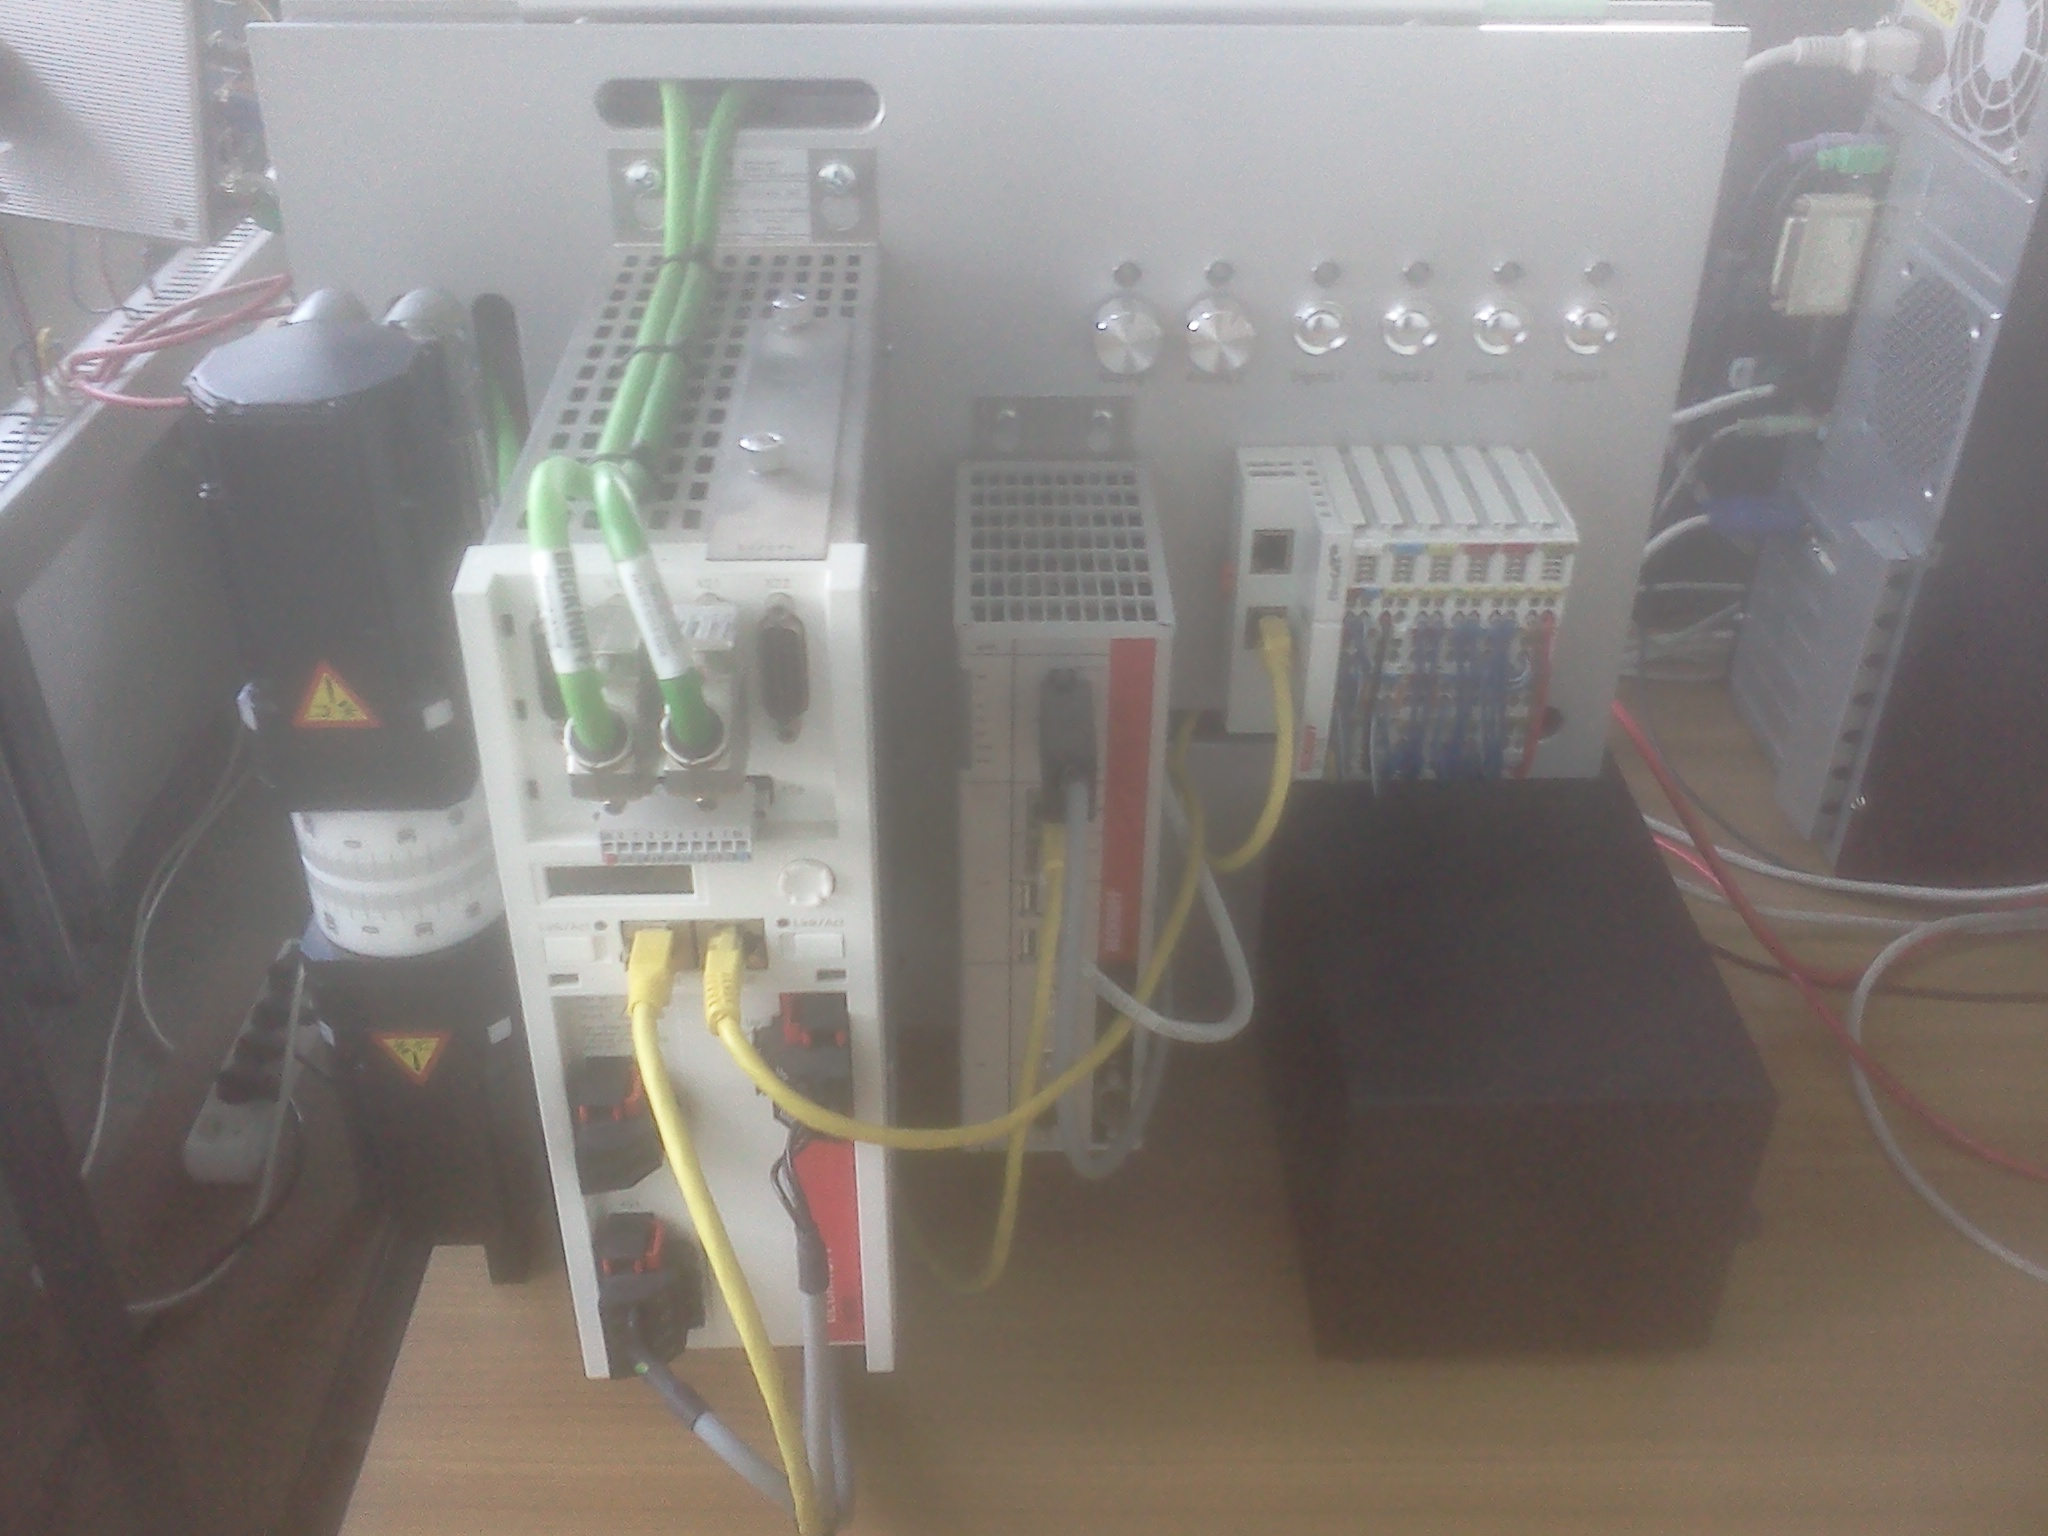
\includegraphics[height=0.8\textheight]{images/typ1.jpg}
\end{figure}
\end{frame}

\begin{frame}
\frametitle{Stanowisko typ 1}
\begin{enumerate}
    \item 2 silniki AM3021-0C00-0000
    \item Wyspa EK1100 z zestawem modułów IO
    \item Napęd serwomechnizmów AX5203(2 osiowy napęd)
    \item Komputer przemysłowy C6925
    \item Zasilacz
\end{enumerate}
\end{frame}

\begin{frame}
\frametitle{Stanowisko typ 2}
\begin{figure}[!htb]	
\centering 	          
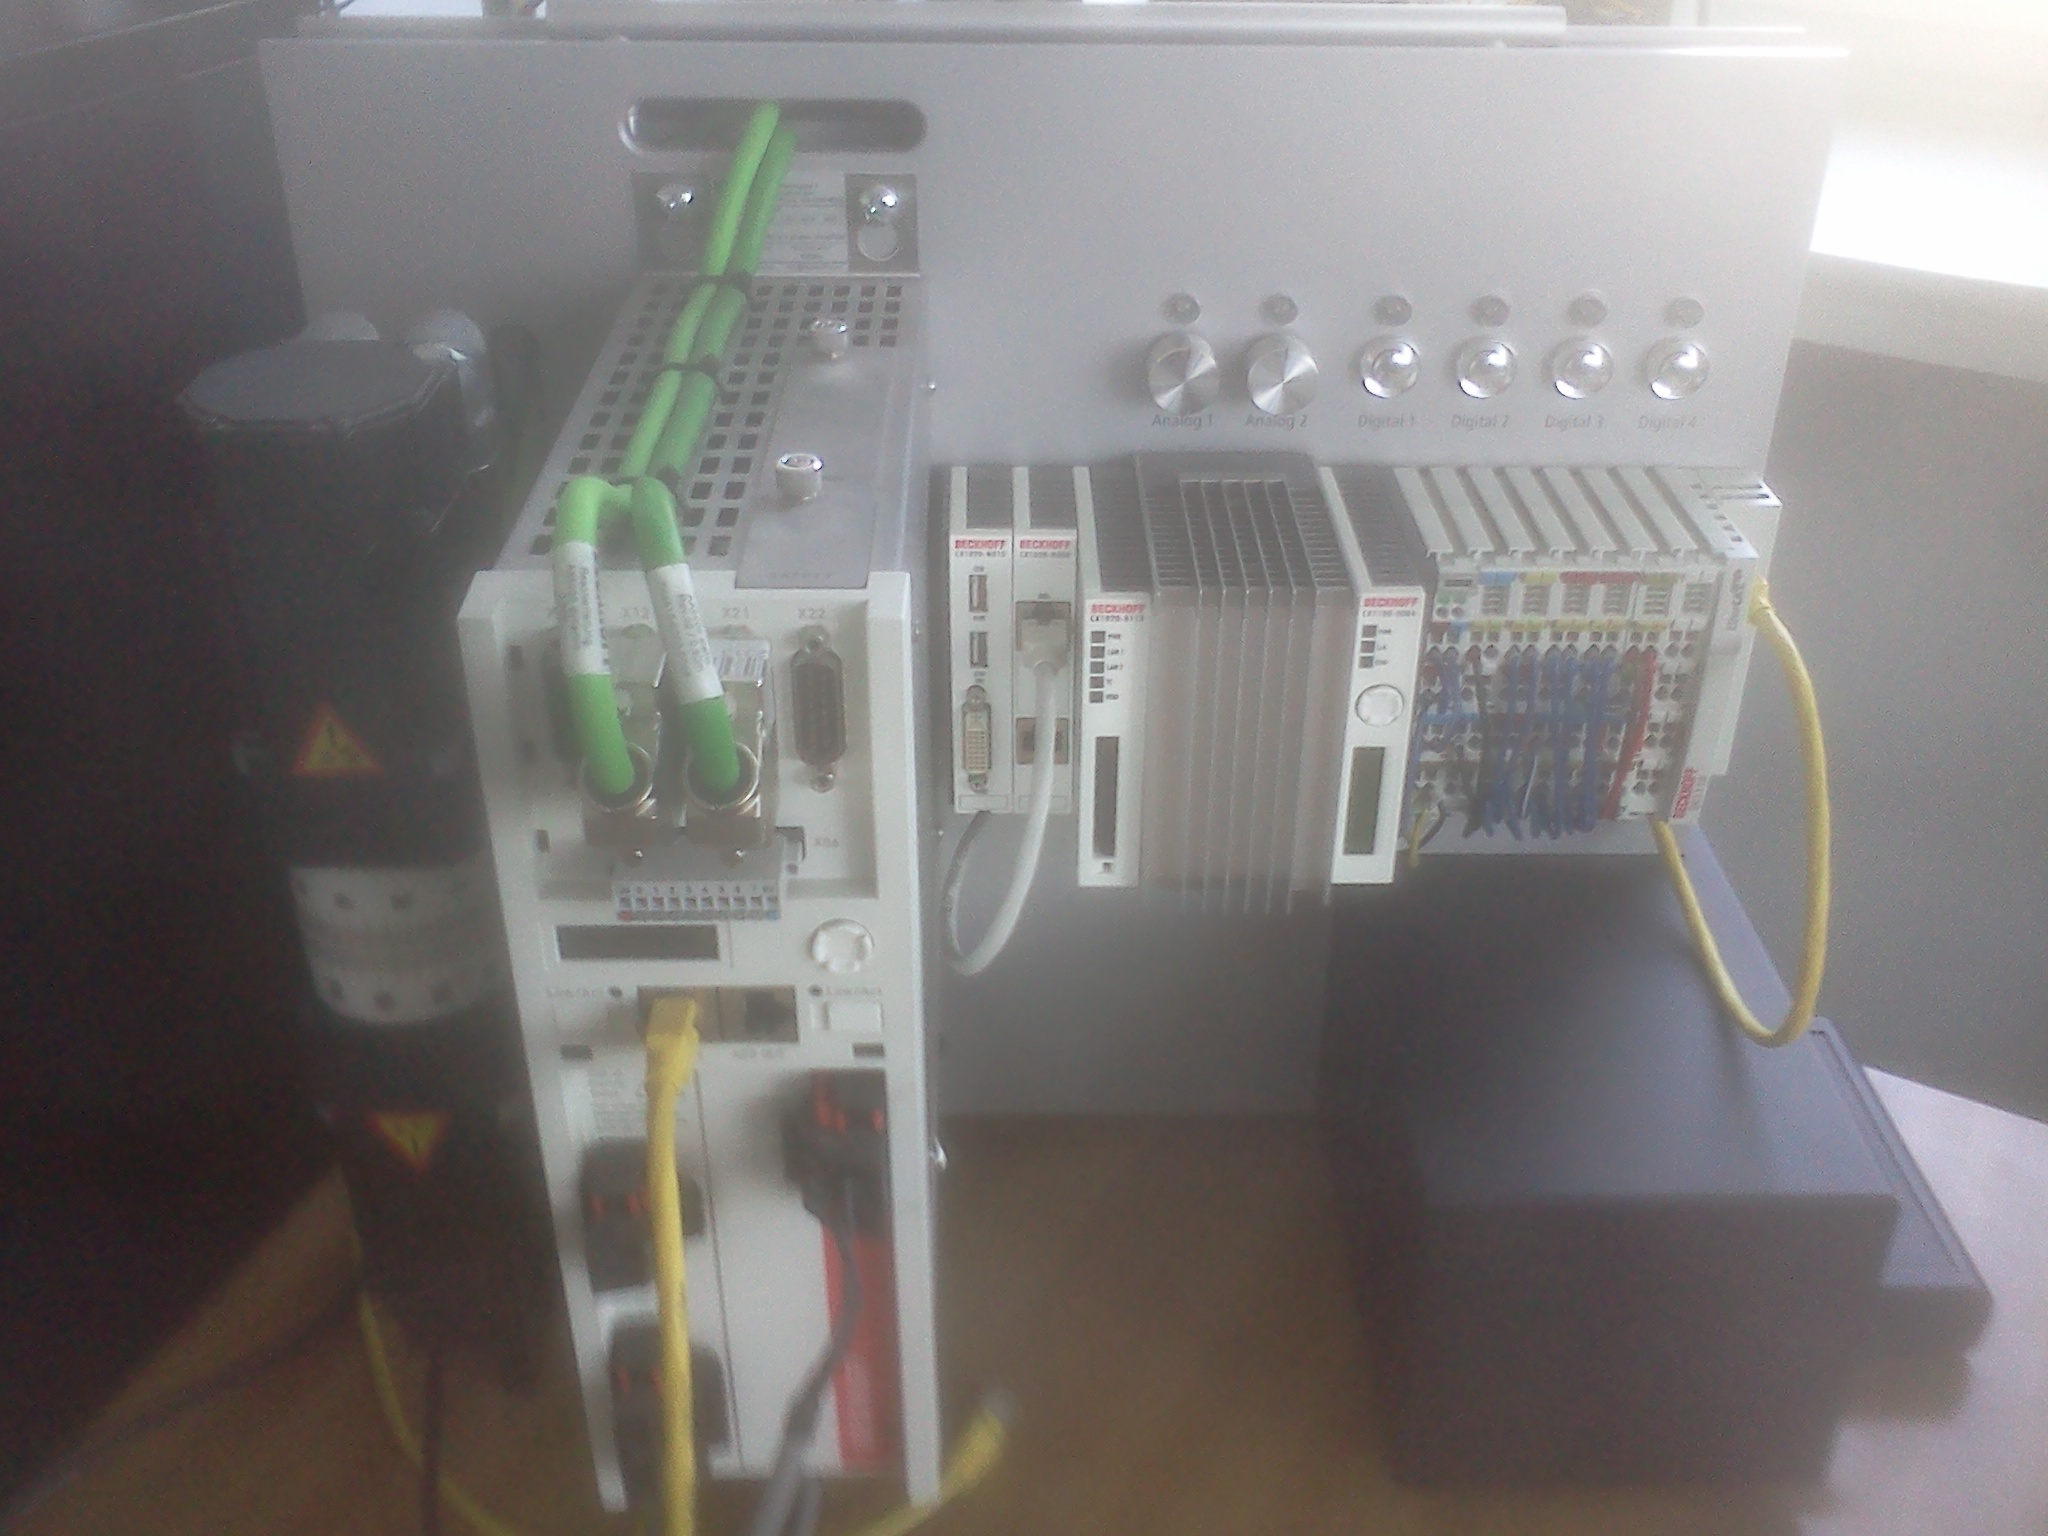
\includegraphics[height=0.8\textheight]{images/typ2.jpg}
\end{figure}
\end{frame}

\begin{frame}
\frametitle{Stanowisko typ 2}
\begin{enumerate}
    \item 2 silniki AM3021-0C00-0000
    \item Wyspa EK1100 z zestawem modułów IO
    \item Napęd serwomechnizmów AX5203(2 osiowy napęd)
    \item Modułowy komputer przemysłowy CX1020
    \item Zasilacz
\end{enumerate}
\end{frame}

\section{Postępy}
\begin{frame}
\frametitle{Co zostało zrobione}
\begin{enumerate}
    \item Konfiguracja systemu dla wszystkich 4 stanowisk
    \item Implementacja projektu na sterownik PLC pozwalającego przetestować działanie konfiguracji, tj. obsługa przycisków, diod, regulację prędkości obrotowej poprzez potencjometr
    \item Rozwiązane problemy o których była mowa na poprzednim seminarium
\end{enumerate}
\end{frame}

\begin{frame}
\frametitle{Główny widok projektu}
\begin{figure}[!htb]	
\centering 	          
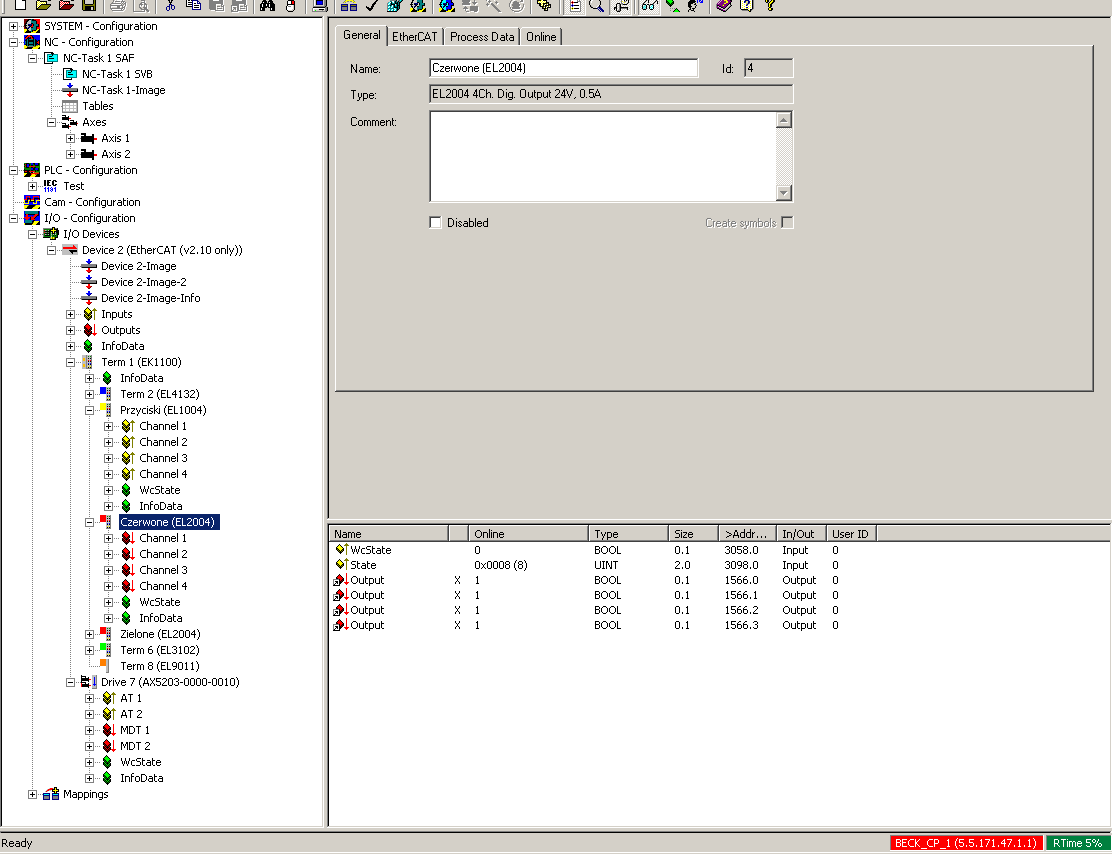
\includegraphics[width=1.04\textwidth]{images/main_view}
\end{figure}
\end{frame}

\section{Problemy}
\begin{frame}
\frametitle{Rozwiązane problemy}
\begin{enumerate}
    \item Problem z uruchomieniem jednego silnika - nie wykrywany przez system
    \item Problem z uruchomieniem automatycznym projektu po restarcie stanowiska - pomimo konfiguracji analizy działania w testach.
\end{enumerate}
\end{frame}

\subsection{Problem 1}
\begin{frame}
\frametitle{Konfiguracja osi A}
\begin{figure}[!htb]	
\centering 	          
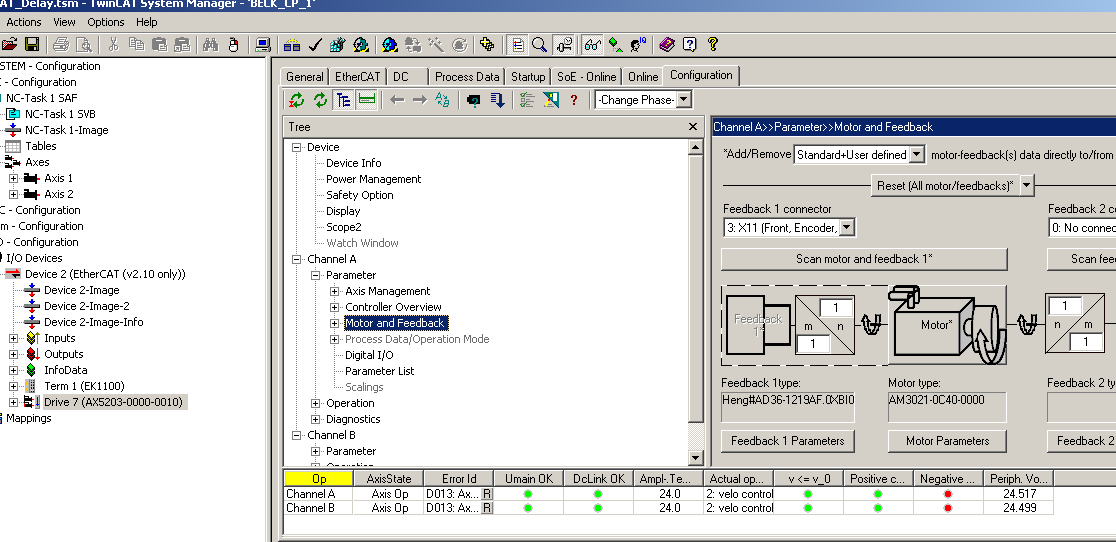
\includegraphics[width=1.04\textwidth]{images/config_axis1}
\end{figure}
\end{frame}

\begin{frame}
\frametitle{Konfiguracja osi B}
\begin{figure}[!htb]	
\centering 	          
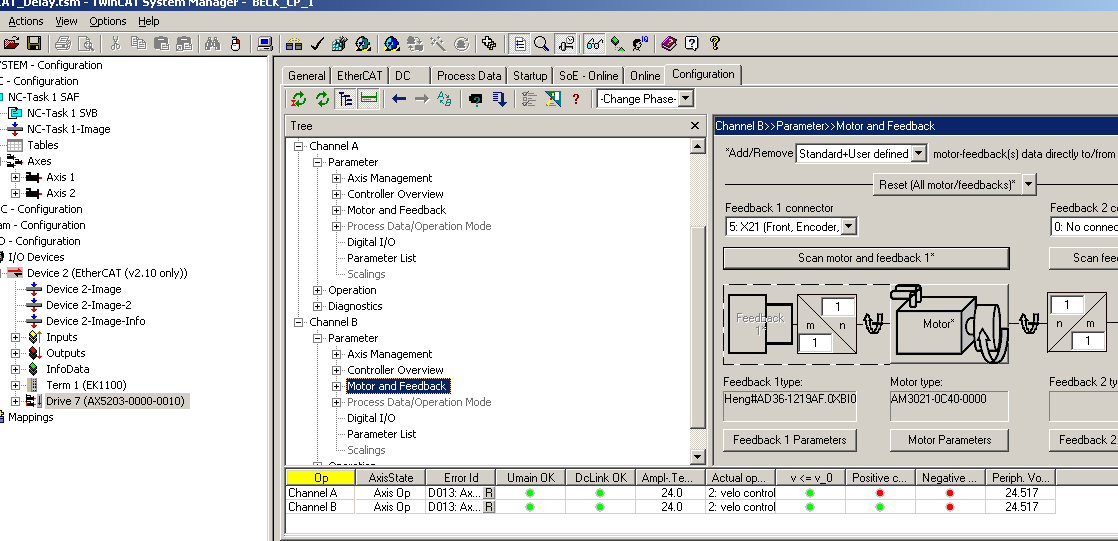
\includegraphics[width=1.04\textwidth]{images/config_axis2}
\end{figure}
\end{frame}

\begin{frame}
\frametitle{Działanie osi A}
\begin{figure}[!htb]	
\centering 	          
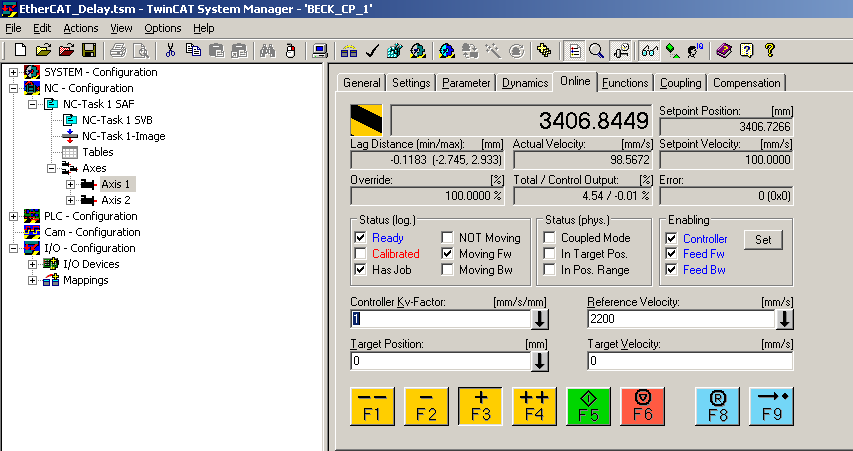
\includegraphics[width=1.04\textwidth]{images/axis1}
\end{figure}
\end{frame}

\begin{frame}
\frametitle{Działanie osi B}
\begin{figure}[!htb]	
\centering 	          
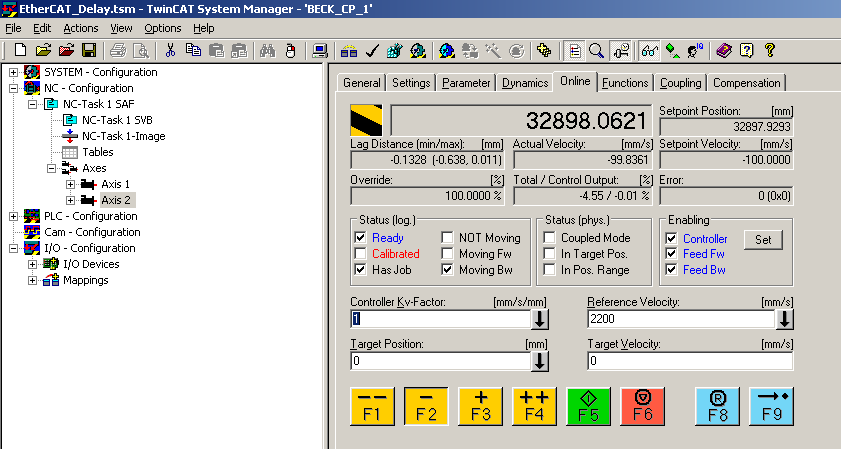
\includegraphics[width=1.04\textwidth]{images/axis2}
\end{figure}
\end{frame}

\subsection{Problem 2}
\begin{frame}
\frametitle{Stworzenie bootowalnego projektu}
\begin{figure}[!htb]	
\centering 	          
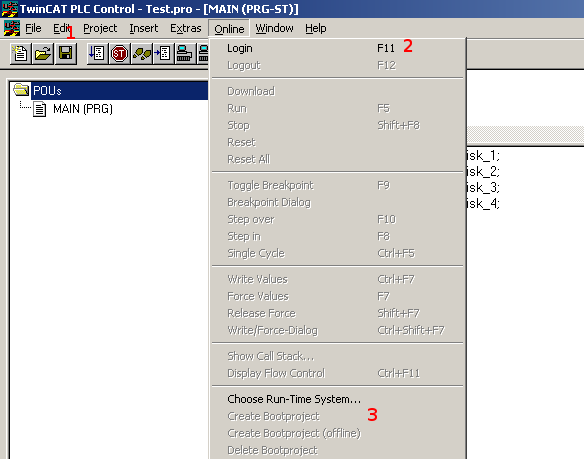
\includegraphics[width=1.0\textwidth]{images/boot}
\end{figure}
\end{frame}

\begin{frame}
\frametitle{Stworzenie bootowalnego projektu}
\begin{enumerate}
    \item Zbudowanie projektu:
    \begin{itemize}
		\item Edit
		\item Rebuild all
	\end{itemize}
    \item Zalogowanie do sterownika (Login)
    \item Stworzenie bootowalnego projektu (Create Bootproject)
    
\end{enumerate}
\end{frame}

\section{Podsumowanie}
\begin{frame}
\frametitle{Aktualny stan pracy}
\begin{enumerate}
    \item Przygotowanie aktualnego projektu do przeprowadzenia badań
    \item Przeprowadzenie zaplanowanych badań
    \item Dokończenie książki
\end{enumerate}
\end{frame}

\begin{frame}
\frametitle{Pytania}
Czas na pytania.
\end{frame}

\begin{frame}
\frametitle{Podsumowanie}
Dziękuję za uwagę.
\end{frame}

\end{document}